
\documentclass[journal, 11pt]{IEEEtran}

\usepackage[utf8]{inputenc}
\usepackage[english]{babel}
\usepackage{graphicx}

% \usepackage{amsmath, amsthm, amssymb, amsfonts}
% \usepackage{algorithm}
% \usepackage{algpseudocode}
% \usepackage{minted}
\usepackage{booktabs}
\usepackage[colorlinks=true, linkcolor=red, urlcolor=cyan, citecolor=red]{hyperref}
% \usepackage[numbers]{natbib}
% \setcitestyle{authoryear,open={[},close={]}} %Citation-related commands

% correct bad hyphenation here
\hyphenation{op-tical net-works semi-conduc-tor}


\begin{document}
%
% paper title
% Titles are generally capitalized except for words such as a, an, and, as,
% at, but, by, for, in, nor, of, on, or, the, to and up, which are usually
% not capitalized unless they are the first or last word of the title.
% Linebreaks \\ can be used within to get better formatting as desired.
% Do not put math or special symbols in the title.
\title{Human-Machine Dialogue Project\\AI Cooking Assistant}
%
%
% author names and IEEE memberships
% note positions of commas and nonbreaking spaces ( ~ ) LaTeX will not break
% a structure at a ~ so this keeps an author's name from being broken across
% two lines.
% use \thanks{} to gain access to the first footnote area
% a separate \thanks must be used for each paragraph as LaTeX2e's \thanks
% was not built to handle multiple paragraphs
%

\author{Rigo Andrea}
        % \{username1, username2\}@domain.com}% <-this % stops a space


% note the % following the last \IEEEmembership and also \thanks - 
% these prevent an unwanted space from occurring between the last author name
% and the end of the author line. i.e., if you had this:
% 
% \author{....lastname \thanks{...} \thanks{...} }
%                     ^------------^------------^----Do not want these spaces!
%
% a space would be appended to the last name and could cause every name on that
% line to be shifted left slightly. This is one of those "LaTeX things". For
% instance, "\textbf{A} \textbf{B}" will typeset as "A B" not "AB". To get
% "AB" then you have to do: "\textbf{A}\textbf{B}"
% \thanks is no different in this regard, so shield the last } of each \thanks
% that ends a line with a % and do not let a space in before the next \thanks.
% Spaces after \IEEEmembership other than the last one are OK (and needed) as
% you are supposed to have spaces between the names. For what it is worth,
% this is a minor point as most people would not even notice if the said evil
% space somehow managed to creep in.



% The paper headers
\markboth{Human-Machine Dialogue  @ Trento university 2022}%
{}
% The only time the second header will appear is for the odd numbered pages
% after the title page when using the twoside option.
% 
% *** Note that you probably will NOT want to include the author's ***
% *** name in the headers of peer review papers.                   ***
% You can use \ifCLASSOPTIONpeerreview for conditional compilation here if
% you desire.




% If you want to put a publisher's ID mark on the page you can do it like
% this:
%\IEEEpubid{0000--0000/00\$00.00~\copyright~2015 IEEE}
% Remember, if you use this you must call \IEEEpubidadjcol in the second
% column for its text to clear the IEEEpubid mark.



% use for special paper notices
%\IEEEspecialpapernotice{(Invited Paper)}




% make the title area
\maketitle

% As a general rule, do not put math, special symbols or citations
% in the abstract or keywords.


% Note that keywords are not normally used for peerreview papers.
% \begin{IEEEkeywords}
% IEEE, IEEEtran, journal, \LaTeX, paper, template.
% \end{IEEEkeywords}






% For peer review papers, you can put extra information on the cover
% page as needed:
% \ifCLASSOPTIONpeerreview
% \begin{center} \bfseries EDICS Category: 3-BBND \end{center}
% \fi
%
% For peerreview papers, this IEEEtran command inserts a page break and
% creates the second title. It will be ignored for other modes.
\IEEEpeerreviewmaketitle








% \section*{Summary} %Longer + must be only on Rotation Averaging
% Abstract


\section{Introduction}
This project builds a small demo conversational agent with the aim of helping the user cook a recipe, following it step by step. The user can directly select a recipe (assuming that it is present in the assistant database) or ask the system to propose some recipes. After a recipe is selected, the system will read the ingredient list for the user, and will help to follow the steps by telling him/her what the current step is, then switching to next step when the user finished the current one and tells the system to proceed.
Additionally, the system can manage a shopping list for the user and handle some basic chitchat.
The system is task based, designed to help the user in some predefined tasks such as following a recipe, adding and removing items from a shopping list and handle chitchat on a basic level.
The recipe database is hand-written and the assistant is build on top of the Rasa framework \cite{rasaframework} version 2.8.17.
This report describes the tasks the system is designed to carry out in section \ref{sec:domain}, the dialogues that the system can handle in section \ref{sec:conv-design}, the model used in section \ref{sec:pipeline}, the data in section \ref{sec:data-desc} and the evaluations techniques and results in section \ref{sec:eval}.
The code is available on \href{https://github.com/andrearigo-dev/cooking-assistant-hmd}{the GitHub repository}.

\section{Domain}
\label{sec:domain}
As mentioned in the introduction, the system can handle three main tasks:
\begin{itemize}
    \item Cooking assistance
    \item Shopping list management
    \item Chitchat and FAQs
\end{itemize}

\subsection{Cooking assistance}
The user can ask the model to suggest a recipe, for example by saying \textit{"What can I cook today?"}.
The system will then display a list of recipes for the user to choose from. Since the database only contains four recipes, the code will currently display all of them. If the assistant would be subject of further development it would have to be adjusted to display a random selection of recipes.
The assistant will then guide the user to fill the required slots to start cooking a recipe: the desired recipe itself and the number of people the user would like to cook for.
A more experienced user that already knows which recipes the system knows can directly select a recipe and number of people, for example Carbonara, by saying \textit{"Let's cook Carbonara"} or \textit{"I would like to cook Carbonara for two"}.
Recipes are treated as sequences of steps, where the user can move as he/her sees fit.
By default the system will move to the next step when the user communicates that the current step is done; but the user can ask the system to repeat the current step, go back any number of steps, for example to check for mistakes, while a more experienced user can skip any number of steps if, for example, he/she already knows how to prepare most of the recipe.
Since in some cases the ingredient list can be relatively long and hard to memorize, the user may request the system to repeat the recipe's ingredients.
This can either be done with \textit{"Tell me the ingredients"} to get the entire ingredient list, or by saying \textit{"How much guanciale?"} to request the amount of a single ingredient.
The user can also ask for the amount of an ingredient used in the current step without specifying which one, for example using \textit{"How much of it?"} as input.
In this case the model will look in the database for which ingredient is used in the step and provide the amount. If more than one ingredient is used it will list them and ask the user to disambiguate.

\subsection{Shopping list management}
The system maintains a shopping list for the user that can survive across conversations. For the scope of the project the list is not permanently saved to disk, but it will stay in memory when issuing the \texttt{\textbackslash restart} command as long as Rasa's action server is running.
The shopping list is a simple list of ingredients. The user can ask to see it by saying \textit{"Read my shopping list"}. Since the assistant is supposed to be used with a voice interface and having a voice assistant read a very long shopping list to you can quickly become annoying as it will take a long time, the list is organized in pages, each one will contain five entries.
The user can ask the system to read a specific page, for example by saying \textit{"Read me page three of my list"}.
Based on the user input the system can add to the shopping list a single ingredient, the ongoing recipe (i.e. the user could plan to cook the same thing again, and therefore he/she would need the same ingredients) or any other recipe in the database.
For the latter the model will guide the user to fill the required slots to select a recipe to add.
The last action in this task is removing items from the list. When reading the grocery list the system will prefix each item with a progressive identification number, i.e. \textit{"1 500 grams of pasta"}, then \textit{"2 250 grams of butter"} and so on. The user can then specify the item to be removed by its ID, for example by saying \textit{"Remove item two from my list"} to remove item two.

\subsection{Chitchat and FAQs}
This task is implemented in order to make the assistant able to handle some simple out of domain requests, such as \textit{"How are you?"}, \textit{"Tell me a joke"} or \textit{"Are you a bot?"}.
Chitchat intents are handled by grouping them under a single Retrieval Intent \cite{rasachatfaqs} which is then linked to the proper responses using a single rule \cite{rasarules}.
The chitchat intents that the model can handle are just a few.
However, adding more intents and responses is very easy and doesn't require to add more rules.
This task also handles a few FAQs, questions the user can ask about the system own features. For example \textit{"What can you do for me?"} or \textit{"How do I use the shopping list?"}.

\subsection{User Group}
The target users are home cooks who like to cook for passion or just for necessity.
The audience therefore are people of any gender in the age range of 16-80.


\section{Conversation Design}
\label{sec:conv-design}
The system can handle requests to start a new task, either selecting a recipe to cook or a recipe to add to the shopping list. In this case it will activate a form and guide the user to retrieve the necessary information: the desired recipe and the number of people the user is cooking for.
Once the user has requested a recipe, the assistant will compare it to the recipes in the database using a simple string similarity metric to find the closest match. If no match is found, i.e. the user requested a recipe that is not present in the database, the system will try to recover by suggesting some recipes and ask the user to select another one.
All the other requests are directives in which the users asks for an action to be performed, for example adding an ingredient to the list or to repeat a step, and the machine will perform the action and reply. This type interaction doesn't need a form as the required information is assumed to be in the directive.
The user takes the initiative by directly selecting a recipe or requesting a recipe suggestion. Then the machine takes the initiative by querying the user to gather the information necessary to start a recipe.
Once a recipe is selected, the system guides the conversation by describing a step and the user only has to notify the system when the current step is completed.
However, even if a recipe is running the user can take the initiative at any time by starting another task, or asking the system to perform another action. For example while the cooking task is ongoing the user may ask to add another recipe's ingredients to the shopping list, starting a different task.
The initiative is therefore mixed.
The number of people to cook for, the number of steps to skip or backtrack, the shopping list page number, item IDs and ingredient amounts are all handled by a single entity \texttt{number}.
This is because from a data point of view they are identical and this could confuse the model if they were handled as distinct entities, especially in a project like this where NLU data is scarce.
A simple custom entity extractor allows the model to understand that sentences like \textit{"Just for me"} and \textit{"Skip this step"} that don't explicitly provide a number refer to the \texttt{number} entity of value 1.
While selecting a recipe the system will guide the user to collect the necessary information.
It will then ask for an explicit confirmation, for example: \textit{"I understand you'd like to cook Carbonara for two people, is it right?"}.
While an implicit confirmation is preferable for longer forms, an explicit confirmation is applicable in a case like this, where the required slots are just two.
If the user replies that it's not correct, the system will make him/her fill the slots again. 
Alternatively the user can directly change her mind at any point. For example, assume that user selected Carbonara for two people and the system is asking for the explicit confirmation as discussed previously. She/he can change mind by saying \textit{"Actually I'm going to cook Amatriciana"} to switch to Amatriciana from Carbonara as indicated previously.
In this example, the system will remember the number of people to cook for, and switch to Carbonara without asking the number again.
Adding a recipe's ingredients to the shopping list also activates a form to select a recipe to add but since it requires the same slots as the form to select a recipe to cook, it works exactly in the same way.
The user may also require to stop the current recipe or even opt out of an ongoing form by saying \textit{"Stop this recipe"} or just \textit{"Stop this"}.
The conversation is composed of user directives and machine guidance when the system requires information.
Turn taking is therefore fairly simple, with the user and system replying to each other depending on the current task.
To help novice users the assistant will suggest how to initiate some task, action or a question that the user can ask (a FAQ) to get information on how to use some functionality.
For example, when replying to a greeting such as \textit{"Hi!} the agent will reply with \textit{"Hey! I'm your cooking assistant, you can ask me what I can do at any time!"} directing the user to ask what the system can do, discovering how to use the system.
If the user asks to see his/her shopping list and it turns out to be empty the system will suggest how to add an item to it. When a recipe preparation starts and the system lists the ingredients, it will also tell the user that it is possible to ask it to repeat the ingredient list or the amount of a single ingredient and that the user can also skip steps or backtrack as desired.
Similarly, when describing a recipe's step, the model will also ask the user to tell it when to proceed. Because in longer recipes the corresponding sentence \textit{"Let me know when you are ready for the next step"} would be repeated several times, this might annoy the user. Therefore the assistant asks it only for the first three steps, then it will output just the step description as by now the user should know how to tell the machine to go on to the next step.
The assistant also uses some conversation markers when running an action requested by the user, like \textit{"Great"}, \textit{"Ok"} and \textit{"Sure"} followed by the output.
In case the model is not able to understand the user's input it will trigger a fallback rule that will ask the user to rephrase.
Similarly if the model is not able to predict the proper action to execute, i.e. the prediction confidence is too low, it will utter \texttt{utter\_default} asking the user to rephrase.
The model is also able to understand a limited set of out-of-scope questions that are not part of the domain the assistant operates in, for example \textit{"What's the capital of Italy?"} and will reply by telling the user that it can't help with that question since it's only designed to help in cooking.
Finally, the system is capable to handle two simple cases of ambiguous input. If the user activates the recipe selection form and tries to select two recipes at once or provides two different numbers of people to cook for at the same time, the system will tell the user that it can only handle one recipe at a time, or that only one number of people should be selected.


\section{Conversation Model}
\label{sec:pipeline}
The assistant is built on top of the Rasa framework and uses its default suggested pipeline \cite{rasasuggestedconf}. It employs Rasa's Memoization Policy \cite{rasamempol}, Rule Policy \cite{rasarulepol} and TED Policy \cite{rasated}.
The Memoization Policy remembers the stories from the training data and checks if the current conversation matches them. If so, it will predict the next action from the matching stories.
The TED (Transformer Embedding Dialogue) Policy is a multi-task transformer \cite{tedpol} that recognizes entities and predicts the next action based on the conversation history.
The Rule Policy handles conversation parts that follow a fixed behavior and makes predictions based on any rules in the training data. As described before, here rules are used to implement the fallback mechanisms and chitchat.
The Fallback Classifier \cite{rasafallbackclassf} classifies a message as \texttt{nlu\_fallback} when the NLU confidence is too low, in this case the threshold is the default 0.3.
A rule is then used to activate \texttt{utter\_fallback} whenever \texttt{nlu\_fallback} is predicted.
Similarly, when a message is classified as out-of-scope, a rule activates \texttt{utter\_out\_of\_scope}, telling the user that the assistant can't help with the query.
As for chitchat, when a message is classified a such a rule activates the Response Selector \cite{responsesel} component, that predicts the appropriate response from a set of candidates. The assistant can handle 13 chitchat intents.
The suggested NLU pipeline is composed of:

\begin{itemize}
    \item Whitespace Tokenizer: Creates a token for every whitespace separated character sequence.
    \item Regex Featurizer: Creates a vector representation of user messages using regular expressions. It creates a list of regular expressions, then for each of them a feature will be set marking whether this expression was found in the user message or not.
    \item Count Vector Featurizer: Creates bag-of-words representation of user messages, intents, and responses.
    \item Dual Intent Entity Transformer (DIET) Classifier \cite{diet}: A multi-task architecture for intent classification and entity recognition.
\end{itemize}

The assistant can only run in a terminal and be used via text. Ideally it would be used via voice and it would run through a custom Alexa skill in an Alexa-enabled device, or any other voice-enabled device such as Google Home, but I didn't have any such device at my disposal.
If it were to be further developed to be integrated with such devices, some minor changes might have to be made. For example in Alexa systems the \texttt{stop} intent would be unnecessary as all Alexa skills already have a similar intent, \texttt{AMAZON.StopIntent} \cite{rasatoalexa}, by default.


\section{Data Description and Analysis}
\label{sec:data-desc}
Collecting data for this project was fairly easy thanks to Rasa Interactive \cite{rasainteractive} which allows to interact with assistant while annotating inputs, then saves the conversation as a story and its NLU data.
Rasa also allows to set checkpoints in stories which connect any story ending in a checkpoint to any story starting from the same checkpoint. This allows to easily fork and combine different story blocks, making writing longer stories much easier. Using this technique 135 stories were collected.
The NLU data is composed of 20 distinct intents with an average of 33.7 examples each, for a total of 674 examples.
Synonyms are employed to map spoken numbers like \textit{"two hundreds"} to their numerical values.
The system uses eight slots and four entities: the recipe, the number of people to cook for, ingredients and ingredient's unit, for example grams, kilos and so on.
The recipes database was hand-written just for this project and it only contains four recipes, with an average of 4.75 ingredients and 10.75 steps per recipe.
Since the project only serves as a proof of concept, the database is encoded directly in a Python file, in a format similar to JSON composed of nested dictionaries: the database is a dictionary where each key is a recipe name, and each entry is a recipe.
Each recipe is itself a dictionary that contains a list of steps and a list of ingredients.
Each ingredient is a dictionary containing the name, amount and unit of the represented ingredient.
Each step is a dictionary containing the step description and a list of numbers pointing to the ingredient list entries corresponding to the ingredients used in the step.


\section{Evaluation}
\label{sec:eval}
The system was evaluated using both intrinsic evaluation and extrinsic evaluation.
The intrinsic evaluation is integrated in Rasa, while for the extrinsic one a human evaluation was performed.

\subsection{Intrinsic Evaluation}
NLU intrinsic evaluations were carried out using the K-fold cross validation technique for more accurate results, with \textit{k} set to 5.
For this system's NLU pipeline Rasa's evaluation procedure \cite{rasatest} computes accuracy, F1 score and precision for the intent classification, entity extraction and response selection tasks.
Tables \ref{tab:intent-eval}, \ref{tab:entity-eval} and \ref{tab:chitchat-eval} show the results of intent classification, entity extraction and response selection (chitchat) respectively.
Figures \ref{fig:intent-conf-mat}, \ref{fig:ents-conf-mat}, and \ref{fig:resp-sel-conf-mat} show the intent, entities and response selector confusion matrices respectively.
Additionally, Rasa tests the assistant with test stories and computes the accuracy at story level (i.e. how many stories are completed correctly) and at action level (i.e. how many times the TED policy predicted the correct action).
Both accuracies are 1, as all test stories are completed correctly.
As can be seen from the evaluation results, the assistant performs fairly well. However it's worth noting that the assistant was both trained and evaluated on conversations written by me, not on real conversations collected from human subjects.
Since I knew how the assistant was supposed to work while I was writing training and test stories, the evaluation is inherently biased.
Additionally, although the model achieves good scores, from the confidence distributions of the three NLU tasks, shown in figures \ref{fig:intent-hist}, \ref{fig:ents-hist}, and \ref{fig:resp-sel-hist}, can be observed that the system does some mistakes with high confidence. This means that the NLU data should be improved and expanded to reduce the mistakes the system does.

\begin{table}[ht]
    \centering
    \begin{tabular}{@{}cccc@{}}
        \toprule
        \textbf{} & \textbf{Accuracy} & \textbf{F1 Score} & \textbf{Precision} \\ \midrule
        Train     & 1                 & 1                 & 1                  \\
        Test      & 0.960             & 0.957             & 0.959              \\ \bottomrule\\
    \end{tabular}
    \caption{Intent evaluation results}
    \label{tab:intent-eval}
\end{table}

\begin{table}[ht]
    \centering
    \begin{tabular}{@{}cccc@{}}
        \toprule
        \textbf{} & \textbf{Accuracy} & \textbf{F1 Score} & \textbf{Precision} \\ \midrule
        Train     & 1                 & 0.999             & 0.999              \\
        Test      & 0.996             & 0.983             & 0.992              \\ \bottomrule\\
    \end{tabular}
    \caption{Entity extractor evaluation results}
    \label{tab:entity-eval}
\end{table}

\begin{table}[ht]
    \centering
    \begin{tabular}{@{}cccc@{}}
        \toprule
        \textbf{} & \textbf{Accuracy} & \textbf{F1 Score} & \textbf{Precision} \\ \midrule
        Train     & 0.984             & 0.984             & 0.985              \\
        Test      & 0.804             & 0.790             & 0.815              \\ \bottomrule\\
    \end{tabular}
    \caption{Response selection (chitchat) evaluation results}
    \label{tab:chitchat-eval}
\end{table}

\subsection{Extrinsic Evaluation}
Human evaluation is very important in the evaluation of AI assistants since it allows to observe how the system performs when used by the end user in a real world scenario.
For this project the assistant was tested by three people for as long as they'd liked. They were then asked to answer seven questions, rating from 0 to 10 their experience while using the assistant.
The results are shown in table \ref{tab:human-eval}.
The results are relatively good, but some of the subjects used sentences that were never seen by the assistant during training and it wasn't able to generalize to them. This is also reflected on the relatively low rate on the ability of the system to understand the user as shown on the table.
It also doesn't perform well in the chitchat task but that's to be expected since it is handled with simple rules and the chitchat queries it is designed to understand are just a few.

\begin{table}[ht]
    \centering
    \begin{tabular}{@{}cc@{}}
        \toprule
        \textbf{Question}                                                           & \textbf{Rate (0 to 10)} \\ \midrule
        Rate the system's ability\\ to help you follow a recipe                     & 8                       \\
        Rate the system's ability\\ to help you manage a shopping list              & 8,34                    \\
        Rate the system's ability\\ to do chitchat conversation                     & 5,84                    \\
        Rate how close is this\\ conversation to a conversation with a human        & 6,84                    \\
        Rate the speed of the system\\ in solving the task in comparison to a human & 8                       \\
        Rate the system's ability to understand you                                 & 6,5                     \\
        Were the system responses clear and helpful?                                & 7,5                     \\ \bottomrule\\
    \end{tabular}
    \caption{Human evaluation results}
    \label{tab:human-eval}
\end{table}


\section{Conclusion}
The assistant developed in this work is simple but can successfully manage a shopping list and help the user follow a recipe step by step.
It performs quite well as long as the user sticks to sentences and conversations that appear in the training set, but it fails to generalize to unseen data.
It could be improved by letting many more users use it and collecting the conversations in order to make both NLU data and training stories much larger and more diverse.
It could also be possible to employ pre-trained components in the NLU pipeline, such as spaCy's \cite{spacy} tokenizer, featurizer and entity extractor, which could lead to better performance since they were pre-trained on a much larger volume of data than what was used in this project.


% \nocite*
\bibliographystyle{ieeetr}
% \bibliographystyle{plainnat}
% \bibliographystyle{apalike}
\bibliography{bib}


% large figures
\onecolumn

\begin{figure}[ht]
    \centering
    \includegraphics[width=\textwidth]{figures/intent\_confusion\_matrix.png}
    \caption{Intent confusion matrix}
    \label{fig:intent-conf-mat}
\end{figure}

\begin{figure}[ht]
    \centering
    \includegraphics[width=\textwidth]{figures/entity\_confusion\_matrix.png}
    \caption{Entity confusion matrix}
    \label{fig:ents-conf-mat}
\end{figure}

\begin{figure}[ht]
    \centering
    \includegraphics[width=\textwidth]{figures/response\_selection\_confusion\_matrix.png}
    \caption{Response selection (chitchat) confusion matrix}
    \label{fig:resp-sel-conf-mat}
\end{figure}

\begin{figure}[ht]
    \centering
    \includegraphics[width=\textwidth]{figures/intent\_histogram.png}
    \caption{Intent prediction confidence histogram}
    \label{fig:intent-hist}
\end{figure}

\begin{figure}[ht]
    \centering
    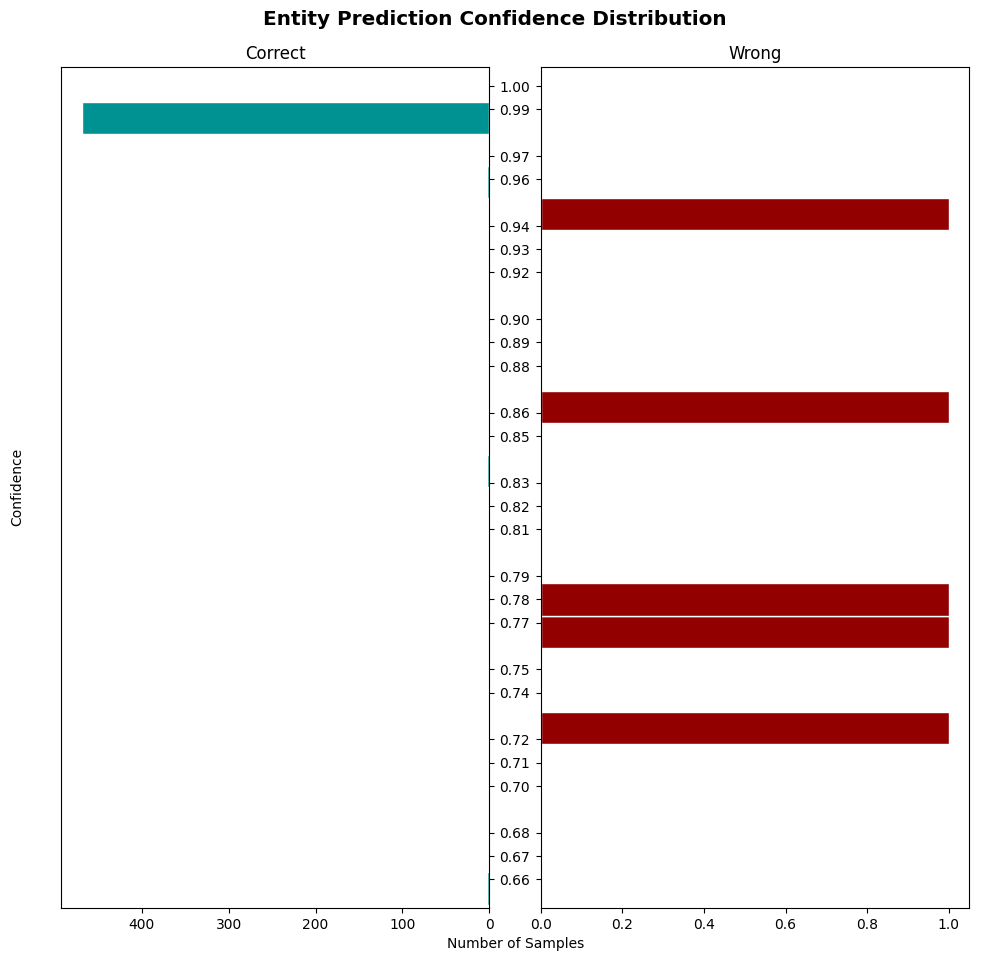
\includegraphics[width=\textwidth]{figures/DIETClassifier_histogram.png}
    \caption{Entity prediction confidence histogram}
    \label{fig:ents-hist}
\end{figure}

\begin{figure}[ht]
    \centering
    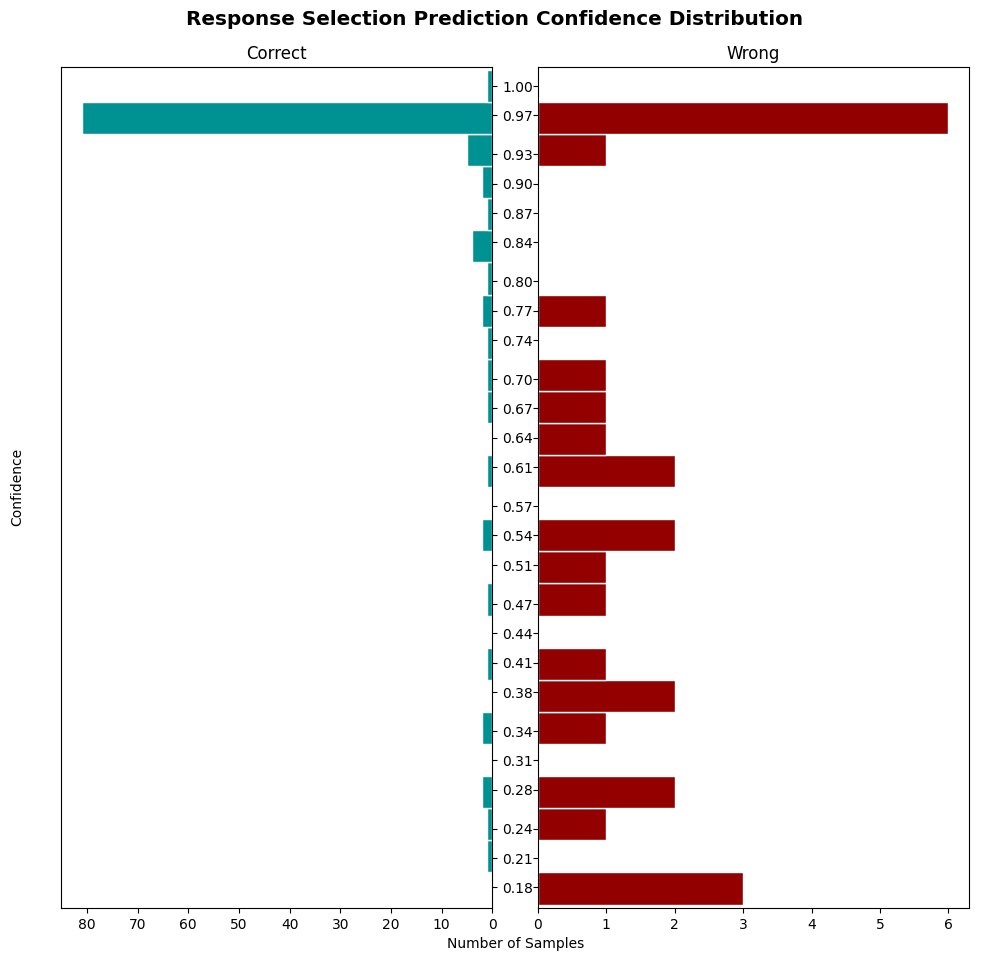
\includegraphics[width=\textwidth]{figures/response_selection_histogram.png}
    \caption{Response selection (chitchat) confidence histogram}
    \label{fig:resp-sel-hist}
\end{figure}


% Can use something like this to put references on a page
% by themselves when using endfloat and the captionsoff option.
\ifCLASSOPTIONcaptionsoff
  \newpage
\fi




\end{document}


